\chapter{Implementation}
\section{Communication}
\paragraph{Every thing has a start and an end} I started my internship September 22nd in Boston. While being on-site and I learned how Acquia manages processes and works together with the community in order to reach business goals. Also watching them work with a lot of remote employees was already a very valuable lesson. More about this experience can be read in the article I wrote about this. Since my involvement with the project there are about 3000 websites using the Drupal 7 version of the module and about 11000 users in total using the module (Drupal 6 and Drupal 7). I've committed more than 220 patches to the Apache Solr project and all of them were made and created publicly and I've had help from a whole community when reviewing those on the fly. I will continue working on the module and I will continue motivating people to help out and make the project better as a whole. 

\paragraph{Exposing the work to the public} I have recently given a presentation ‘Drupal Search’ explaining to more than 60 attendees what was done with the module and where it was heading to in Belgium. Lots of open communication has happened within the community in the Apache Solr Issue Queue. In total I have given 5 presentations with a combined total of more then 400 attendants. 

\subsection{Daily communication}
When the thesis/internship started I was a bit unclear how it would work. Working from your home every day, and having a time difference of 6 hours proved to be quite challenging. 

At acquia they use an internal chatserver but also promote alternative ways of communication. During this period I've used Skype, Adobe Connect, Google Hangout, VOIP using my phone's 3G. Joining conference room calls while 50\% of the people were attending the meeting physically and others remotely was also a daily event to look out for.

From October until the end of December I mainly communicated with Peter Wolanin to keep track of the daily work and to clear out any questions or issues that could block my progress. The methodology was similar to a scrum session but more personal. This sheet was divided in 4 main segments.
\begin{itemize}
  \item What did I get done since last meeting.
  \item What will I get done before the next meeting
  \item What is slowing me down or blocking progress
  \item What did you discover that would be of interest, or needs to be discussed post scrum?
\end{itemize}

Below one can see how this looked like. The full document is available upon request. 
\begin{figure}[H]
     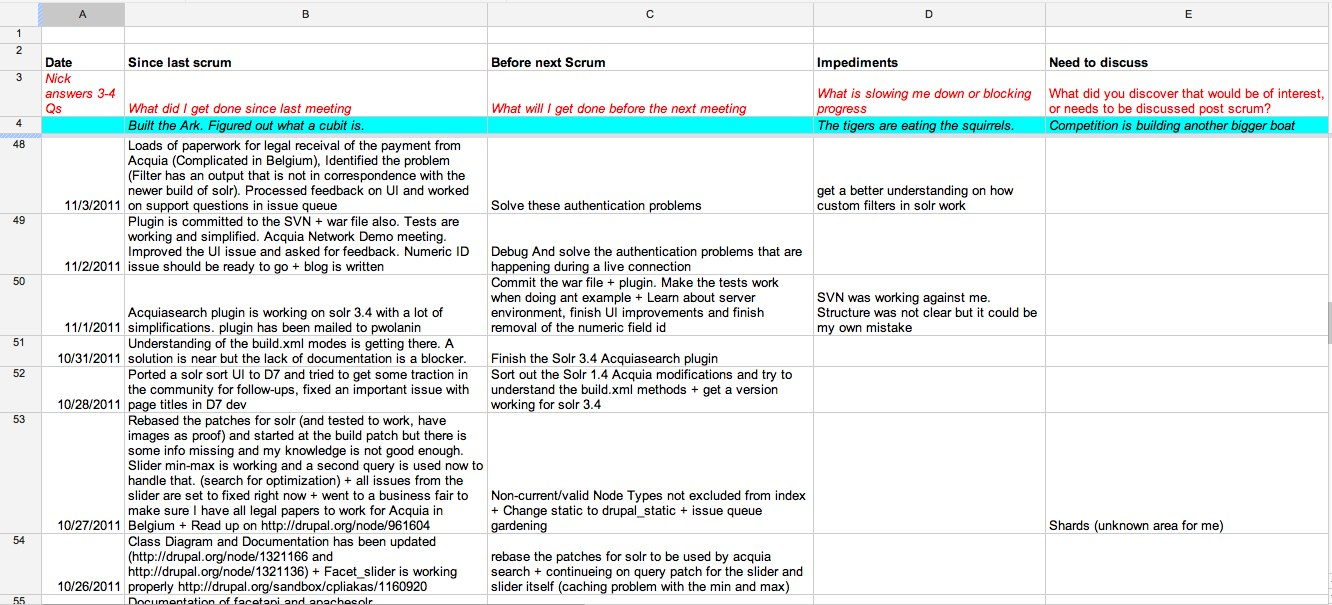
\includegraphics[width=\textwidth]{images/scrum_example_solr.jpg}
     \caption{Mini Daily Scrum worksheet}
\end{figure}

From the 1st of January I also joined the team of Michael cooper, who leads the network project in Acquia. He holds a daily standup where we do a similar exercise but ,instead of writing, the team members tell (preferable while standing up) what they have done, what they plan to do and what is blocking them. The network team uses a full scrum methodology. \footnote{More about scrum can be found here. This section does not elaborate further because since scrum itself could be a whole other thesis.\url{http://en.wikipedia.org/wiki/Scrum_(development)}}

\subsection{Drupal Camps and seminars}
Exposing the work that was done in a community such as Drupal is very important to get validation and also constructive comments to be able to built further. Those meetings (Drupalcamps, DrupalDays, anything similar) are important to meet people that are in the same technologic space. People with experience and knowledge, but also people with an opinion that makes one think, think hard. Also it is important to expose knowledge to people who are new to Drupal, it makes their lives easier and, if all goes well, the community can count on one more skilled person to help out in need. 

After the redesign of the Apache Solr UI and a bunch of other changes under the hood there were a couple of events that accepted a talk from me and allowed me to explain what I did, why I was doing this and how they could help making all of this more successful.
 
\paragraph{Drupal User Group Belgium} The 9th of November I gave a presentation in Ghent, Belgium about Search in Drupal 7. More than 60 attendees showed up and most of them were happy to learn about the details of Search and more about Apache Solr. Details can be found on \url{http://drupal.be/evenement/dug-drupal-user-group-meeting-over-search-in-drupal-7}

\paragraph{Drupal Camp Toulouse} From the 26th of November until the 27th of November I've attended a Drupalcamp in Toulouse \url{http://toulouse2011.drupalcamp.fr/en}. Even though I was not allowed to present as an Acquian member I did go there and I've presented as myself. The topic of the presentation was similar but more focussed on questions and answers. The french audience was a bit smaller (around 30) compared to the Drupal User Group in Belgium but the talks I had afterwards with members of the community were great.

\paragraph{Acquia Internal Training} On the 2nd of December I presented the same presentation as the one I did in Toulouse but then for the employees of Acquia, using an online platform. In the company this is a called a lunch and learn so a bunch of people gather during lunchtime and follow a presentation about a certain topic. Personally this was the most stressful presentation because there was less interaction and I could not see the audience. On the other hand, the audience could not see me neither. The only thing visible was my computer screen and the presentation. Around 15 people attended this presentation. The presentation from Toulouse and the Internal Training can be found on \url{http://prezi.com/j-wss0nznowb/acquia-lunch-and-learn-december-2011-drupal-search/}

\paragraph{Drupal Science Camp} A totally different experience was the Drupal Science Camp in Cambridge. This Camp was organized in 21st and the 22nd of January in a business complex and was crowded. everything was organized really quickly but that did not affect the quality of the conference. I gave a final overview of what I had done in those months and what could/should still happen when my time was over. More information about the session can be found on \url{http://www.drupalsciencecamp.org.uk/sessions/drupal-search-and-solr-wizardry}. Over 40 people were packed in a room to listen to the presentation and approached me with challenging questions. 

\subsection{Blog Posts}
To continue on the dissemination of the results and get an even broader audience a series of blog posts were written. They have generated, when accumulated, over 20.000 page views and a series of comments and reactions.

\begin{itemize}
\item Using Github application in your patch workflow \footnote{\url{http://nickveenhof.be/blog/using-github-application-patch-workflow-0}} 
\item Attending the Boston Drupal User Group \footnote{\url{http://nickveenhof.be/blog/boston-drupal-user-group}} 
\item Changing a git commit message in the commit history \footnote{\url{http://nickveenhof.be/blog/changing-git-commit-message-commit-history}} 
\item A story of an intern at Acquia \footnote{\url{http://nickveenhof.be/blog/story-intern-acquia}} 
\item Adding a custom plugin to Solr \footnote{\url{http://nickveenhof.be/blog/adding-custom-plugin-solr}} 
\item A simple guide to install Apache Solr 3.x for Drupal 7 \footnote{\url{http://nickveenhof.be/blog/simple-guide-install-apache-solr-3x-drupal-7}} 
\item Slides of the Drupal Search and Solr sessions \footnote{\url{http://nickveenhof.be/blog/drupal-search-and-solr-dug-november-2011}} 
\item Upgrading from Apache Solr 1.4 to Apache Solr 3.5 and its implications \footnote{\url{http://nickveenhof.be/blog/upgrading-apache-solr-14-35-and-its-implications}} 
\end{itemize}

\paragraph{Conferences + Blogging Result}
An estimated crowd of 150 people have seen the presentation and the work in front of me and a whole lot more have seen the blog posts. All this from start to end, early and a later stage. By presenting a work often, and exposing what one does quickly, it raises the chance on a better product in the end. All the constructive comments were written down and reported back to the daily scrum and were merged in to the roadmap. This feedback also gave an invaluable pointer to the importance of certain items, such as the multi entity support, in the roadmap. Working remotely removes a lot of physical contact but these social events surely compensate a missing piece in the puzzle for remotes. 

\section{Apachesolr module for Drupal 7 version 7.x-1.0}
The module got a major overhaul in these months. Over 219 commits from the author were made to the codebase of the Apache Solr project 
\subsection{Search Environments}
\paragraph{UI Improvements}
As seen in chapter 4 it became clear that the old UI did not suffice for managing multiple environments. Also there was no way to remove environments and/or clone them. During the process the search environment got its own tab (under settings) and it is also directly visible if a search environment is online or not (green color). 
The advanced configuration got overhauled also and now includes options such as the amount of items to index per cron and also a select box of what to do when the module fails to connect/fails to execute a query. The benefit of having multiple environments is easy. retrieving data from two indexes or having indexes for the development/staging and production environment. 
Another addition that was made is that the search bias and boost information is now environment dependent instead of being applied to all queries.

\begin{figure}[H]
     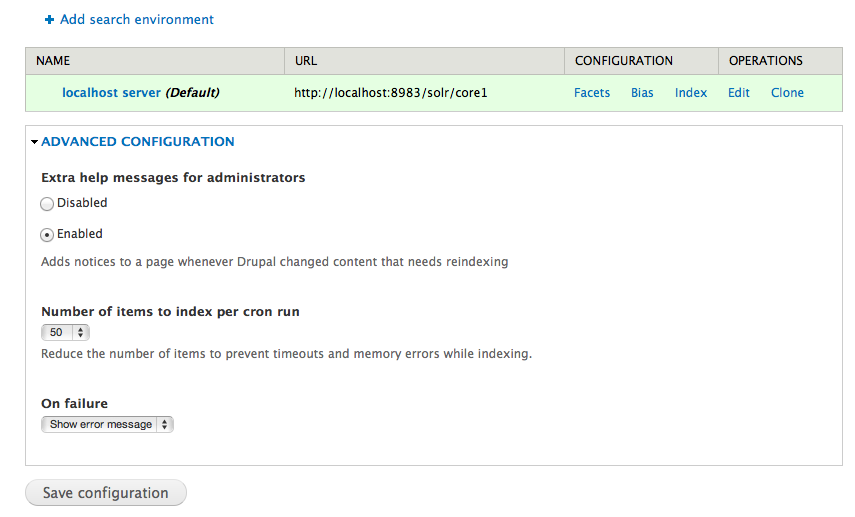
\includegraphics[width=\textwidth]{images/implementation/search_environments.png}
     \caption{Search Environments}
\end{figure}

\paragraph{Functions}
Originally, the module did not have support for multiple search environments. Just moments before this thesis was executed some small support for multiple search environments was added. Most of the functions did not take a search environment argument and were dependent on the default search environment. During these months of dedication to the Apache Solr Module we improved the support for multiple search environments. 

Listing 7 is a list of functions signatures with their parameters. All of them were adjusted to support multiple environments since none of these functions were already supporting this functionality. Changing all of them was a tedious work that involved a lot of testing, feedback and more testing. Which brings you, my dear reader to the next paragraph!
\inputminted[fontsize=\scriptsize,linenos]{php}{./code_examples/functions_environments.php}
\captionof{listing}{List of functions that were modified to support multiple environments}

\paragraph{Testing}
Drupal uses a specific framework for testing, called Simpletest \footnote{Simpletest info can be found on \url{http://drupal.org/simpletest}} This testing framework is nested very deeply into the Drupal 7 development process. 

The Functional tests are the most common. They create a fresh database installation and specifically create data for the test in the database and then make assertions based on expected results. Unit tests work without a database installation in the backend and are useful for isolated functions that don't make assumptions about the larger system. Upgrade tests use a database dump from an earlier version of Drupal and import that to run update.php and then check assertions.

For the search environments tests were written as functional tests. As explained above these test try to assess the functionality from an UI point of view.
\inputminted[fontsize=\scriptsize,linenos]{php}{./code_examples/testEditSearchEnvironment.php}
\captionof{listing}{Example of a search environment test}

\inputminted[fontsize=\scriptsize,linenos]{php}{./code_examples/test_signature_search_environments.php}
\captionof{listing}{All the test signatures concerning the search environments}

\begin{figure}[H]
     
\includegraphics[width=10cm]{images/implementation/test_search_environments.png}
     \caption{In total 227 tests assesments were written in 6 functional tests for the search environments, all of them pass}
\end{figure}

\paragraph{Exportable}
The environments are also exportable to code so that is becomes easier for deployment \footnote{View more about Deployment and Drupal at \url{http://drupalize.me/videos/introduction-drupal-features-module}} to another server-environment. Ctools\footnote{Ctools is a module that is available on \url{http://drupal.org/project/ctools} and is primarily a set of APIs and tools to improve the developer experience} is utilized to help enabling the export of this configuration.  

\subsection{Search pages}
\begin{wrapfigure}{r}{0.5\textwidth}
\begin{center}
     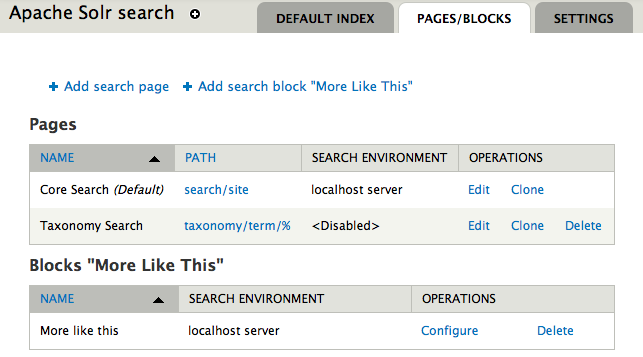
\includegraphics[width=0.5\textwidth]{images/implementation/search_pages_overview.png}
     \caption{Search pages overview page}
\end{center}
\end{wrapfigure}
\paragraph{UI Improvements}Also the Search Pages obtained a massive change UI wise. All the functionality is now merged in to one solid landing page for search pages. The core search page is now a part of the search pages list, whereas before it was a separate process and also separate code. Every search page has a title, a path, a designated environment where it should send its requests to and naturally an edit link, a clone link and a delete link where it is allowed. It is by default not allowed to remove the core search page since this would break the whole process. 
This breakage is due to the dependency on the Search module within Drupal Core. More about that in the next paragraph. 

\begin{wrapfigure}{l}{0.5\textwidth}
\begin{center}
     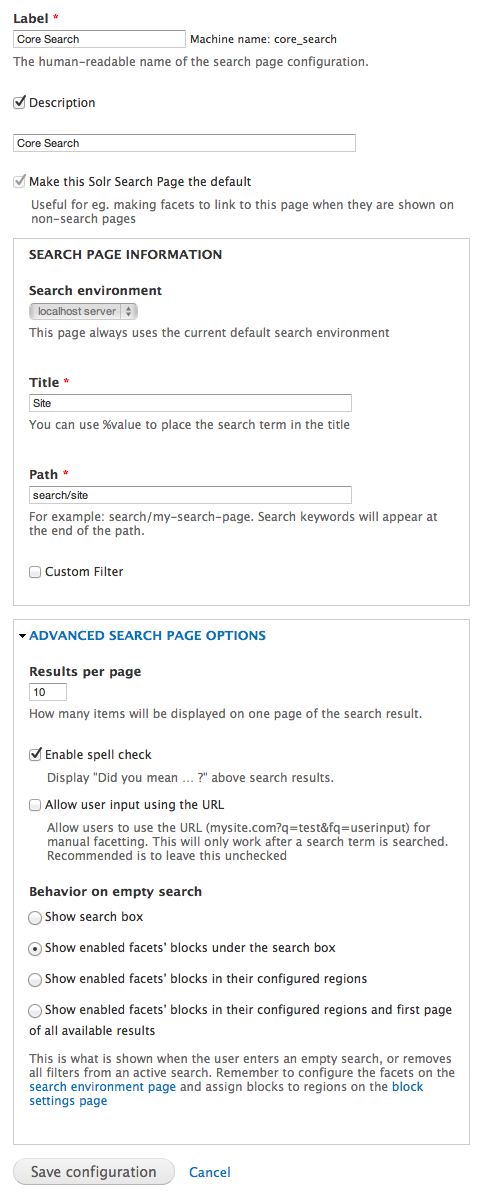
\includegraphics[width=0.5\textwidth]{images/implementation/search_page_detail.png}
     \caption{Search Page Configuration : Label and Description}
\end{center}
\end{wrapfigure}
\paragraph{Edit a Search Page} First and foremost a search page needs a label and optionally a description. A compliant machine name will be automatically generated from the label. Another option that is critical is the question to the site creator if the search page, that is being shown, should be the default search page. This has implications such as to which search page the search block should forward its requests to. 

\paragraph{Search Page Configuration :  Information} What follows is the selection of the search environment. As explained earlier a search environment is a place where the queries can be sent to. Each Drupal site can have multiple search environments if needed. By default it will select the default search environment in the search page configuration. The title field allows the site creator to have a dynamic search title whenever a search is being executed. For example, if a user searches for "Foo", the title of the search results will be : Search results for "Foo". To generate this the site creator should fill in the configuration with "Search results for \%value". Next up is the path, a critical part of the search page since this will be the value that is shown in the URL. For the adventurous site creator there is an option to supply a custom filter. This means that when a search page is created to search within blogs only, the custom filter should have the value "bundle:blog" \footnote{Granted that the content type has a machine name "blog"}. This allows deep customizations to any search page and allows site creators to fine tune their site. Multiple filters can be entered if they are separated with a comma.

\begin{wrapfigure}{r}{0.5\textwidth}
\begin{center}
     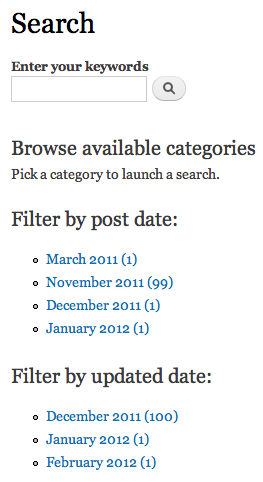
\includegraphics[width=0.3\textwidth]{images/implementation/blocks_under_search_box.png}
     \caption{Setting : Show enabled facets' blocks under the search box}
\end{center}
\end{wrapfigure}
\paragraph{Search Page Configuration : Advanced options}
Most of the settings here as self-explanatory. For instance, one can set the amount of search results per page or enable the spellchecker. It also allows the site creator to allow user input from the URL (\url{mysite.com?q=test&fq=userinput}) for manual faceted search. This will only work after a search term was entered. The recommended course here is to leave this unchecked unless one really knows what he/she is doing. The behavior on empty search setting allows the site creator to choose what to do when an empty search is being executed. Figure 5.6 and Figure 5.7 show the impact of these settings for the end user. 

\begin{figure}
     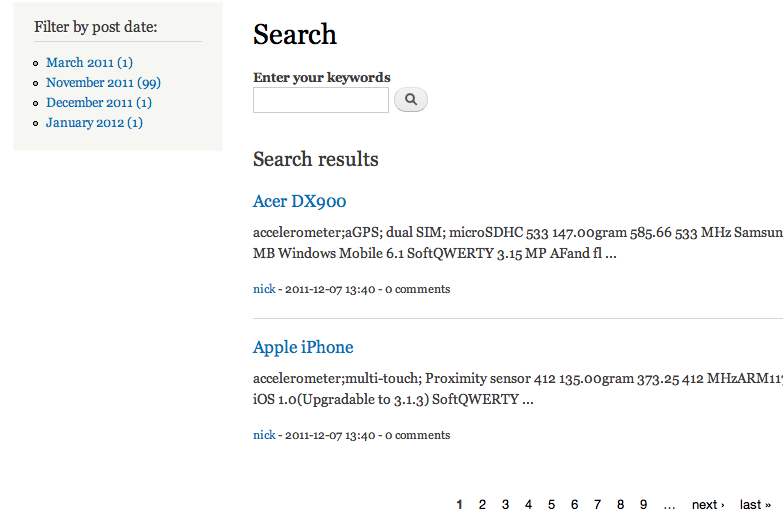
\includegraphics[width=\textwidth]{images/implementation/search_first_page_with_blocks_in_region.png}
     \caption{Setting : Show enabled facets' blocks in their configured regions and first page of all available results. As one can see it looks like a real search, but looking closer to the search box there is no search keyword entered.}
\end{figure}

\paragraph{Functions}
One of the major issues that was resolved is \#1314406 \footnote{\url{http://drupal.org/node/1314406} by Nick\_vh, scor: Fixed De-duplication of the apachesolr\_search\_execute() and apachesolr\_search\_user\_defined\_search\_page().} which made it possible that the core search page is approached in the same was as any custom search page. Listed below are all the 

\inputminted[fontsize=\scriptsize,linenos]{php}{./code_examples/functions_search_pages.php}
\captionof{listing}{All the function signatures that involve the search pages}

\paragraph{Testing}
For the search environments tests were written as functional tests. As explained earlier these test try to assess the functionality from an UI point of view.
\inputminted[fontsize=\scriptsize,linenos]{php}{./code_examples/testEditSearchPages.php}
\captionof{listing}{Example of a search environment test}

\inputminted[fontsize=\scriptsize,linenos]{php}{./code_examples/test_signature_search_pages.php}
\captionof{listing}{All the test signatures concerning the search environments}

\begin{figure}[H]
     
\includegraphics[width=0.8\textwidth]{images/implementation/test_search_pages.png}
     \caption{In total 110 tests assesments were written in 4 functional tests for the search environments, all of them pass}
\end{figure}

\paragraph{Exportable}
Similarly to the Search Environments all search pages are exportable. See Search Environments for a deeper understanding.

\subsection{Query Object}
\paragraph{} This class allows you to make operations on a query that will be sent to Apache Solr. methods such as adding and removing sorts, remove and replace parameters, adding and removing filters, getters and setters for various parameters and more. During the timeframe of this work not a lot of changes were made to this class but some are worthy to mention.

\paragraph{User input validation}
The attached snippet takes care of a half-restrictive validation of user input. This snippet was written by thorough testing and reading up on the essence of regular expression. Gratitude goes out to all that try to explain regular expressions online and to people that helped testing it \footnote \url{http://drupal.org/node/1313698} by Nick\_vh, denikin: Fixed Support for search of multiword content in facets/fields.}. The problem was that a filter as complex as "\url{fq={!cache=false cost=5}inStock:true&fq={!frange l=1 u=4 cache=false cost=50}sqrt(popularity)}" but also a filter as simple as "\url{fq={!bundle:(article OR page)}}" should be validated properly

The function was divided in 4 main parts and the function is also included for closer inspection to those that are interested.
\begin{enumerate}
\item Breaking up the string in to separate parts. The different parts are defined as "name" and "value".
\item Validates the name and the value of the filter
\item Validates opening and closing brackets
\item Validate date value syntax if it is a date.
\end{enumerate}

\inputminted[fontsize=\scriptsize,linenos]{php}{./code_examples/filter_value_regex.php}
\captionof{listing}{Validating user input. Custom filters in search pages or user input from URL}


\begin{wrapfigure}{l}{0.4\textwidth}
\begin{center}
     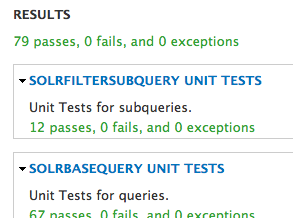
\includegraphics[width=0.4\textwidth]{images/implementation/test_query_subquery.png}
     \caption{In total 79 test assesments were written in 3 unit tests for the search environments, all of them pass}
\end{center}
\end{wrapfigure}
\paragraph{Testing}
Naturally, functionality like this should be tested so mistakes like these do not occur again. To do this a list was set up with good and bad queries.

\subparagraph{Good Combinations}
\begin{packed_itemize}
\item {!cache=false}inStock:true']
\item {!frange l=1 u=4 cache=false}sqrt(popularity)']
\item {!cache=false cost=5}inStock:true']
\item {!tag=impala}model:Impala']
\item {!anything that appears to be local}']
\item bundle:(article OR page)']
\item -bundle:(article OR page)']
\item -{!anything that appears to be local}']
\item title:"double words"']
\item field\_date:[1970-12-31T23:59:59Z TO NOW]'] 
\end{packed_itemize}

\subparagraph{Bad combinations}
\begin{packed_itemize}
\item wrong name:"double words"']
\item field\_date:[1970-12-31 TO NOW]']
\item bundle:((article OR page)]']
\end{packed_itemize}

These test now all report back as succeeded. The test suite for the base query also includes tests such as parsing the filters, adding and removing the filters, adding search keywords to the query and last but not least the support for subqueries \footnote{Subqueries basically allow two query objects to be merged into one}.

\subsection{Entity layer}
\paragraph{Entity support for Drupal 7}
Drupal 7 introduced entities \footnote{Introduction to entities \url{http://drupal.org/node/1261744}}. 
Originally, in Drupal 6 there was only 1 concept and that was content types. In Drupal 7 this changed, thanks to the Entity Api, and it can now add fields to any entity. A content type is an entity now, but also users and terms. An entity is a useful abstraction to group fields. On top of that we have bundles. Bundles are an implementation of an entity type, similar to a subtype of an entity.

Back when the Apache Solr module was first created, there was no such thing as the entity api and the architecture could also not take this change into account. After some time it became apparent that developers wanted to have this native support to fulfill the needs of their clients. During these months a particular issue \footnote{\url{http://drupal.org/node/966796}  by Nick\_vh, scor, BarisW, wesnick, swentel, LSU\_JBob | Crell: Added Separate indexer for multiple entity types.} in the issue queue got a lot of attention. Over 145 comments were made and a bunch of patches were posted. Ultimately the patch got accepted and it opened up perspectives for new entity support in the Apache Solr module. A set of new API functions became available and some modules like apachesolr\_user\_indexing \footnote{\url{http://drupal.org/project/apachesolr_user_indexer}}, apachesolr\_commerce \footnote{\url{http://drupal.org/project/apachesolr_commerce}} and apachesolr\_term \footnote{\url{http://drupal.org/project/apachesolr_term}} are already using the new API possibilities.

\inputminted[fontsize=\scriptsize,linenos]{php}{./code_examples/entity_api.php}
\captionof{listing}{Api functions to support multiple entities}

\subsection{Performance optimizations}
\paragraph{Performance during indexing}
There were a couple issues open in the queue that go back to 2009. One \footnote{\url{http://drupal.org/node/592522} by Nick\_vh, pwolanin | quaoar: Hooks node\_type(), taxonomy and user knocks out our database server.}of them is interesting enough to explain here. Before the problem is explained the reader should be aware that Drupal 7 incorporates a database layer, commonly referred to as DBTNG \footnote{\url{http://drupal.org/developing/api/database}}. The Drupal database layer is built atop PHP's PDO library. PDO provides a unified, object-oriented API for accessing different databases but it does not provide an abstraction for the different dialects of SQL used by different databases.

Exactly this abstraction is strapping us here. MySQL has some flaws that become clear after reading the stackoverflow source \footnote{\url{http://stackoverflow.com/questions/3417074/why-would-an-in-condition-be-slower-than-in-sql/3417190\#3417190}} about in conditions in MySQL. In summary, whenever a query is done in the form of 

\begin{minted}{sql}
SELECT FROM * WHERE TYPE IN(SELECT FROM * WHERE TYPE = "BLOG");
\end{minted}
\caption{Example of a problematic query in MySQL}

it could produce slow results. DBTNG follows the SQL 1999 standard \footnote{\url{http://en.wikipedia.org/wiki/SQL:1999}} and this kind of query is absolutely allowed. So whenever a subquery is used to generate the parameters for the IN set, it could lead to performance problems for MySQL. Most other database backends have resolved this problem already. Since it is known that most servers where Drupal is run are still using MySQL, the module had to be adjusted to solve this problem. 

\paragraph{Different query per database type} After some research was done we found a way to retrieve the same result set but by executing a different query against MySQL. Unfortunately there was no way to write this type of SQL with the DBTNG layer at the moment of the patch because the update query does not support adding extra JOIN's \footnote{\url{http://api.drupal.org/api/drupal/includes!database!database.inc/function/db_update/7\#comment-15459}}. Finally it was decided that an extra query for MySQL would be added and that the program would switch depending on the database type the Drupal website was running on.

\begin{minted}{php}
<?php
/**
 * $table = the table where the indexable nodes are located
 * $account = the account of the user that is indexing
 */
switch (db_driver()) {
  case 'mysql' :
    $table = db_escape_table($table);
    $query = "UPDATE {{$table}} asn
      INNER JOIN {node} n ON asn.entity_id = n.nid SET asn.changed = :changed
      WHERE n.uid = :uid";
    $result = db_query($query, array(':changed' => REQUEST_TIME, 
      ':uid' => $account->uid,
     ));
     break;
   default :
     $nids = db_select('node')
       ->fields('node', array('nid'))
       ->where("uid = :uid", array(':uid' => $account->uid));
     $update = db_update($table)
       ->condition('nid', $nids, 'IN')
       ->fields(array('changed' => REQUEST_TIME))
       ->execute();
}
\end{minted}
\caption{Switching between database types}



\section{Facet Api module for Drupal 7 version 7.x-1.0}
\paragraph{Facet Api} As explained in Chapter 4 there was also some work that was assigned to the author to get a better integration with Facet API. Most of the work was already done by Cpliakas so unlimited gratefulness for him because the module works wonderfully. There were more problems solved and if you want to read all the suggestion is to read the changelog.txt of the module for full details. 

\subsection{Facet Query Types}
\begin{wrapfigure}{r}{0.5\textwidth}
\begin{center}
     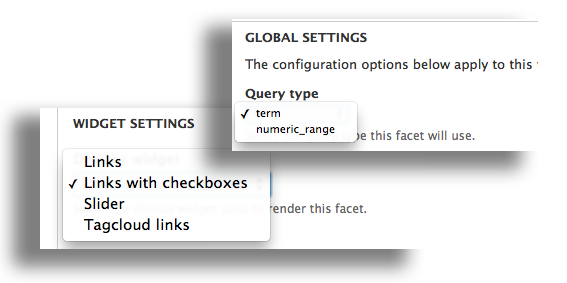
\includegraphics[width=0.5\textwidth]{images/implementation/facet_query_type_and_widget.png}
     \caption{Setting : Query type}
\end{center}
\end{wrapfigure}
\paragraph{}
A query type is in essence a way how Facet API connects with its backend module to provide him data about the facets. Apache Solr has 3 query types
\begin{packed_itemize}
\item Query Type for Terms
\item Query Type for Dates
\item Query Type for Numeric Ranges
\end{packed_itemize}

Each of those already existed in the Apache Solr Module. They might have received a small refinement but in essence they were there. As seen in our class diagram in chapter 4 Facet API has a concept of widgets. Widgets are a visual way in how data is presented to the user. 
The problem existed in the fact that 1 facet could obtain different widgets and as a consequence it should also be able to switch query types. For example, a list of prices (Terms) switches its widget to a slider (Numeric Range). This example was not possible because each field was mapped to only 1 query type.

This was solved by making a one-to-many relationship with query types and their facets. Progress was tracked in an issue \footnote{\url{http://drupal.org/node/1161434} by Nick\_vh, cpliakas: Modify 'query type" key in facet definition to accept an array.} Notice that in the example the "query type" parameter is still present. This is due to the fact that backwards compatibility was important at that stage. Site creators that implement facet can choose either one of them.

\begin{wrapfigure}{l}{0.25\textwidth}
\begin{center}
     \vspace{-25pt}
     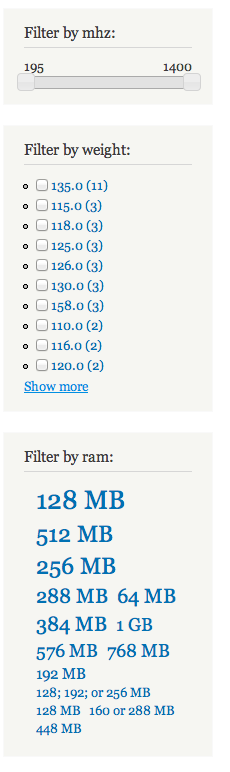
\includegraphics[width=0.25\textwidth]{images/implementation/facetapi_widgets.png}
     \caption{Different widgets in the user interface}
     \vspace{-25pt}
\end{center}
\end{wrapfigure}
\paragraph{}
\begin{minted}{php}
<?php
// Before
'list_integer' => array(
    'indexing_callback' => 'apachesolr_fields_default_indexing_callback',
    'map callback' => 'apachesolr_fields_list_facet_map_callback',
    'index_type' => 'integer',
    'facets' => TRUE,
    'query type' => 'term',
    'facet missing allowed' => TRUE,
  ),

// After
'list_integer' => array(
    'indexing_callback' => 'apachesolr_fields_default_indexing_callback',
    'map callback' => 'apachesolr_fields_list_facet_map_callback',
    'index_type' => 'integer',
    'facets' => TRUE,
    'query types' => array('term', 'numeric_range'),
    'query type' => 'term',
    'facet missing allowed' => TRUE,
  ),
\end{minted}
\caption{A before and after view of the query types key}
\clearpage

\section{Backporting Facet API And Apache Solr to Drupal 6}
Backporting a module from Drupal 7 to Drupal 6 sounds easy but it is not. A programmer is used to all the new tools that are offered to him/her such as the new database layer, some of the Drupal 7 API changes (no more superfunctions \footnote{Superfunctions are functions that try to do it all, in Drupal 7 most of those were replaced with separate functions, hence the big increase in amount of functions}) and most importantly the better theming layer. All progress was also tracked publicly in issue [\#1387164] \footnote{\url{http://drupal.org/node/1387164} by Nick\_vh, gnucifer | cpliakas: Backport Facet API to Drupal 6.} for Facet API and in [\#1387628] \footnote{\url{http://drupal.org/node/1387628} by Nick\_vh: Backport 7.x-1.x to 6.x-3.x.} In this small chapter it tries to explain what was learned from this procedure.

\paragraph{DBTNG to MySQL}
Converting DBTNG was easy at first because there is a wonderful little helper module called DBTNG for Drupal 6. It is a backport of the Drupal 7 PDO database compatibility layer. \footnote{\url{http://drupal.org/project/dbtng}} When everything runs you can start to backport the DBTNG queries to regular MySQL queries. An easy debug function exists in Drupal 7, namely dpq() \footnote{\url{http://api.drupal.org/api/devel/devel.module/function/dpq/7}} that prints out a SQL version of the query object.

\paragraph{Autoload}
Facet Api extensively uses classes and also the autoload functionality of Drupal 7. Drupal 6 does not have this functionality so again a helper module was installed for temporary purposes. This helper module is easily enough called "Autoload" \footnote{\url{http://drupal.org/project/autoload}} and takes care of the lazy loading of classes for you. near the end of february there was a small attempt to get rid of this dependency but there are just too many dynamic classes that it would be better if Autoload stayed. This might be revisited in the near future if Cpliakas decides it should not depend on Autoload.

\paragraph{Static Variables}
Drupal 7 has a concept of dynamic static variables using the drupal\_static method \footnote{\url{http://api.drupal.org/api/drupal/includes!bootstrap.inc/function/drupal_static/7}}. This drupal\_static are statics that are attached to the function instead of the whole project. In Drupal 6 we do not have this concept so in Facet Api the function ctools\_static is used, that mimics this behavior. \footnote{ctools\_static is part of the ctools module}.

\paragraph{Theming layer / Drupal Render}
Drupal 6 handles output very different. While in Drupal 7 everything renders at the end of a complete load, Drupal 6 renders at the level of a specific function. This change was not easy but finally it was quite easy. In the example can be seen that the Drupal 6 version really tries to mimic as much from Drupal 7 as possible. The reason is that when new patches come out for the Drupal 7 version they can be easily integrated/applied to the Drupal 6 version. 

\begin{minted}{php}
<?php
  // Initializes output with information about which server's setting we are
  // editing, as it is otherwise not transparent to the end user.
  $output['apachesolr_index_action_status'] = array(
    '#prefix' => '<h3>' . t('@environment: Search Index Content', array('@environment' => $environment['name'])) . '</h3>',
    '#theme' => 'table',
    '#header' => array('type', 'value'),
    '#rows' => $messages,
  );
  $output[] = //more content in arrays
  return $output;
?>
\end{minted}
\caption{Drupal 7 renderable arrays}

\begin{minted}{php}
<?php
  // Initializes output with information about which server's setting we are
  // editing, as it is otherwise not transparent to the end user.
  // Initializes output with information about which server's setting we are
  // editing, as it is otherwise not transparent to the end user.
  $title = t('@environment: Search Index Content', array('@environment' => $environment['name']));
  $output['apachesolr_index_action_status_prefix'] = '<h3>' . $title . '</h3>';
  $output['apachesolr_index_action_status'] = theme('table', array('type', 'value'), $messages);
    // Print in a similar way as the Drupal 7 version
  $output_print = NULL;
  foreach ($output as $print) {
    $output_print .= $print;
  }
  return $output_print;
?>
\end{minted}
\caption{Drupal 6 Direct output}

\paragraph{Entity to Content Type}
Doing a backport of the whole entity support to support of only 1 entity type "node" with bundles was challenging. Certainly if most of the API functions don't exist in Drupal 6. This was solved by letting Apache Solr for Drupal 6 depend on the CCK project \footnote{Content Construction Kit \url{http://drupal.org/project/cck}}. By doing this every content type in Drupal 6 got the possibility of adding extra information to it. This allowed the module to add callbacks to specific "bundles" in the same way as Drupal 7 did with entities and bundles. Learning by example is the best so a comparison is included between Drupal 7 and 6 for a function that allows a specific entity\_type to reindex. In Drupal 6 there is only 1 entity\_type available and that is "node".

\begin{minted}{php}
<?php
function apachesolr_index_mark_for_reindex($env_id, $entity_type = NULL) {
  foreach (entity_get_info() as $type => $entity_info) {
    if (($type == $entity_type) || ($entity_type == NULL)) {
      if ($entity_info['apachesolr']['indexable']) {
        $bundles = apachesolr_get_index_bundles($env_id, $type);
        $reindex_callback = '';
        if (!empty($bundles)) {
          $reindex_callback = apachesolr_entity_get_callback($type, 'reindex callback');
        }
 ...
}\end{minted}
\caption{Drupal 7 version for indexing a specific entity type for reindexation.}

\begin{minted}{php}
<?php
function apachesolr_index_mark_for_reindex($env_id, $entity_type = 'node') {
  foreach (content_types() as $content_type => $entity_info) {
    if (!empty($entity_info['extra']['apachesolr']['index'])) {
      $reindex_callback = apachesolr_entity_get_callback($entity_type, 'reindex callback');
    }
...
\end{minted}
\caption{Drupal 6 Port of the same function, using content\_types. A function from CCK}

\section{Acquia Search Upgrade from 1.4 to 3.x}
As clarified earlier, Acquia Search is the hosted search solution of Acquia. They provide first class support to customers that do not want to maintain their Apache Solr servers. They also take care of security and previously an employee of Acquia wrote an extension for Apache Solr 1.4 to add the HMAC authentication. This HMAC authentication was added by using a Java Filter Servlet. 
\paragraph{The problem} However, Acquia Search needed to keep up with the latest stable version of Apache Solr which is 3.5. When the Java Filter Servlet was applied to Apache Solr 3.5 it did not work. 
Acquia wanted to hire an external consultant at first to fix the problem but fortunately a solution was found.

\subsection{Java Filter Servlet}
in Solr 1.4, response.getWriter() was used by the SolrDispatchFilter for any character based responses – but in version of Solr 3.4+, because of the issues related to SOLR-2381 \footnote{\url{https://issues.apache.org/jira/browse/SOLR-2381}}, SolrDispatchFilter was modified to use response.getOutputStream() for both binary and character based streams.

The filter that was written only had support for the getWriter method so support had to be added for the getOutputStream method. Without going much into detail a servlet was written in a couple of days that supported this. It took a lot of sweat because of unfamiliarity with Java code and more specifically with the Solr Source code but using the issue queue of the Solr project and the help from core Solr developers, who admittedly saw that the author was a beginner in the area \footnote{\url{https://issues.apache.org/jira/browse/SOLR-2878}}, a servlet was written that supported this new getOutputStream. One of the biggest aha-moments was to change the ResponseWrapper to inherit the getOutputStream method. 
\begin{minted}{java}
response.setCharacterEncoding("UTF-8");
PrintWriter out = response.getWriter();
CharResponseWrapper wrapper = new CharResponseWrapper(
  (HttpServletResponse) response);
 
  chain.doFilter(request, wrapper);
  String responseBody = wrapper.toString();
 
  //write the outgoing header
  response.setHeader("Pragma", "hmac_digest=" +
    buildResponseHmac(authenticator, responseBody, s) + ";");
 
  out.write(responseBody);
  out.close();
\end{minted}
\caption{A snippet of the original Acquia HMAC Filter for Solr 1.4}

\begin{minted}{java}
CharResponseWrapper newResponse = new CharResponseWrapper(
    (HttpServletResponse) response);
    
// CharResponseWrapper is responsible for the getWriter and
// getOutputStream support.

chain.doFilter(request, newResponse);
// The response works with byteArrays so we do to

byte[] responseBody = newResponse.getBytes();
// Write the outgoing header with the ByteArray (Performance)

response.addHeader("pragma", "auth=" +
    buildAuthentication(responseBody) + ";");
// Force the encoding to UTF-8 since we know Drupal works with UTF-8
response.setCharacterEncoding("UTF-8");
response.getOutputStream().write(responseBody);
response.getOutputStream().flush();
\end{minted}
\caption{A snippet of the Acquia HMAC Filter for Solr 3.5. The buildAuthentication returns the value that is embedded in the HTTP headers so the client can verify the validity of the response}

\subsection{Performance testing}
\paragraph{Merge Policies} Drupal is an application that has very deep integration with the Apache Solr application and is updating Solr during cron runs (every 30 minutes for example). This does imply that the indexing speed should not be very high but the search speed should be. Apache Solr has a concept of segments (your index is spread over multiple segments) and if a search is executed it needs to gather all these segments and search them. Logically, more segments = slower results.
Solr 1.4 already had some MergePolicy's such as LogByteSizeMergePolicy \footnote{\url{http://lucene.apache.org/java/3_2_0/api/all/org/apache/lucene/index/LogByteSizeMergePolicy.html}} and LogDocMergePolicy \footnote{\url{http://lucene.apache.org/java/3_2_0/api/all/org/apache/lucene/index/LogDocMergePolicy.html}}. 
Solr 3.5 came with a new default MergePolicy and that required some testing to see if this new MergePolicy (TieredMergePolicy \footnote{\url{http://lucene.apache.org/java/3_2_0/api/all/org/apache/lucene/index/TieredMergePolicy.html}}) could be trusted and what effect it has on existing Drupal indexes.
More information regarding these merge policies can be found online at \url{http://java.dzone.com/news/merge-policy-internals-solr}.

\paragraph{Summary of the testing procedure}
\begin{packed_enumerate}
\item Load existing index files in to a new core.
\item Extract Documents from this index
\item Use the extracted documents to insert them in a clean and new core with different configuration
\item Re-run the access log of that subscription for the searches, repeat this twice, use 10000 queries per access log and discard everything except the select queries and repeat this process 3 times to make sure we have a balanced result set
\end{packed_enumerate}

\paragraph{Charts and extra legend information}
\begin{packed_itemize}
\item S14 stands for Solr 1.4
\item S35 stands for Solr 3.5
\item LB stands for Load Balancer
\item SL stands for Slave, this means that the attack happened from the LB to the SL (these results happened 3 times for to contain less variable delays)
\item MA stands for Master, this means that the attack happened from the LB to the MA (these results happened 3 times for to contain less variable delays)
\item MergeFactor for LogbyteMerge and LogDocMerge is set to 4
\item Default means the Default merge policy, Solr 1.4 this is LogByteMergePolicy and for Solr 3.5 this depends on the LuceneMatchVersion
\item L35 means that Lucene has been set to Lucene 3.5 instead of the default
\item When Lucene 3.5 is set for Solr 3.5 and no merge policy was set, this defaults to TieredMergePolicy
\item When Settings is defined, it applies to specific TieredMergePolicy settings
\begin{packed_enumerate}
\item maxMergeAtOnce says how many segments can be merged at a time for "normal" (not optimize) merging
\item segmentsPerTier controls how many segments you can tolerate in the index (bigger number means more segments)
\end{packed_enumerate}
\end{packed_itemize}

\paragraph{Specifications of the test machines}
\subparagraph{Specifications of the Master}
\begin{packed_itemize}
\item Large Instance
\item 7.5 GB memory
\item 4 EC2 Compute Units (2 virtual cores with 2 EC2 Compute Units each)
\end{packed_itemize}

\subparagraph{Specifications of the Slave}
\begin{packed_itemize}
\item High-CPU Medium Instance
\item 1.7 GB of memory
\item 5 EC2 Compute Units (2 virtual cores with 2.5 EC2 Compute Units each)
\end{packed_itemize}

\paragraph{Results}

\begin{figure}
     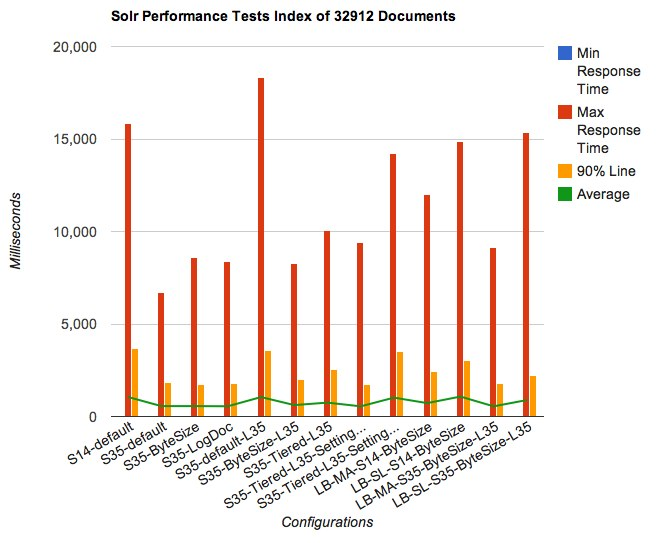
\includegraphics[width=\textwidth]{images/implementation/big-speed.jpg}
     \caption{Speed of quering after a indexing a site with 32912 Documents}
\end{figure}
\begin{figure}
     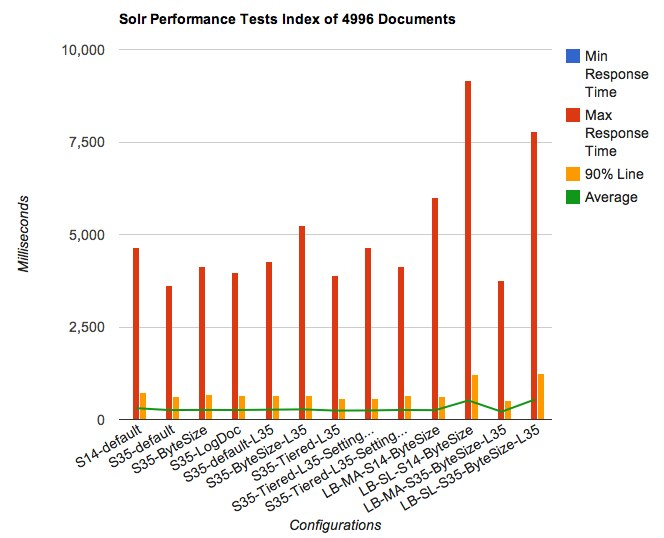
\includegraphics[width=\textwidth]{images/implementation/small-speed.jpg}
     \caption{Speed of quering after a indexing a site with 4996 Documents}
\end{figure}
\begin{figure}
     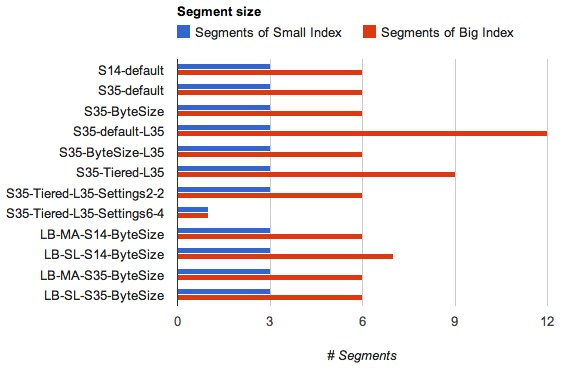
\includegraphics[width=\textwidth]{images/implementation/segments_0.jpg}
     \caption{Size of the segments for all the different test results}
\end{figure}

\paragraph{Conclusions}
If one wants to migrate to Solr 3.5 coming from Solr 1.4 with low risk of changes you should keep using the LogByteMergePolicy with a merge-factor of 4 (Default in the Drupal configs). 
However, the TieredMergePolicy is interesting when understood correctly. For a better understanding more investigation should be done. 

The big outcome of this test is that Solr 3.5 versus 1.4 is a big performance win. Also it is good to know that the MergePolicy should be set explicitly when using LuceneMatchVersion in the solrconfig.xml. This exact conclusion and result is also publicly available on the blog of the Author at \url{http://nickveenhof.be/blog/upgrading-apache-solr-14-35-and-its-implications}.
\clearpage

\section{Additional Modules created to empower users to use the Apache Solr Module suite}
\subsection{Facet Api Slider}
\begin{wrapfigure}{r}{0.4\textwidth}
\begin{center}
     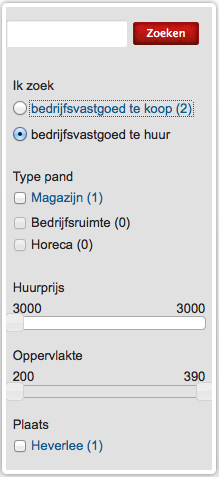
\includegraphics[width=0.4\textwidth]{images/implementation/facetapi_dataflow.png}
     \caption{A real life use case of the Facet Api Slider, implemented by Dataflow \url{http://dataflow.be/}}
\end{center}
\end{wrapfigure}
\paragraph{Use and reason}
The Facetapi Slider \footnote{\url{http://drupal.org/project/facetapi_slider}} was created to make maximum use of the range query type. It allows site creators to easily switch the UI from a list of numeric values to a slider where one can set the minimum and the maximum and the search will be filtered within this range. 

Creating it was not very easy since we had to keep the minimum and the maximum for the global set and also the values that were set by the user. Creating a usable experience proved difficult and there are still discussions \footnote{\url{http://drupal.org/project/issues/facetapi_slider}} ongoing how to improve this process. 

\subsection{Apache Solr Term}
\paragraph{}The Apache Solr Term module \footnote{\url{http://drupal.org/project/apachesolr_term}} provides basic indexing of the taxonomy terms. It makes use of the new entity indexer that was pushed in to the Apache Solr module and allows site creators to index terms, with attached fields. But moreover, users can search for terms.

\subsection{Apache Solr Commerce}
\paragraph{}The Apache Solr Term module \footnote{\url{http://drupal.org/project/apachesolr_commerce}} provides basic indexing of commerce entity types. It makes use of the new entity indexer that was pushed in to the Apache Solr module and allows site creators to index items that are for sale, including their price, with attached fields. When combined with the Facetapi Slider it makes up for a powerful experience in a webshop.

\begin{wrapfigure}{r}{0.4\textwidth}
\begin{center}
  \vspace{-25pt}
   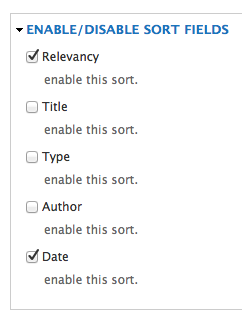
\includegraphics[width=0.4\textwidth]{images/implementation/apachesolr_sort.png}
   \caption{Apache Solr Sort UI sort selection}
\end{center}
\end{wrapfigure}
\subsection{Apache Solr User}
\paragraph{}The Apache Solr User module \footnote{\url{http://drupal.org/project/apachesolr_user}} provides basic indexing of the user entities. It makes use of the new entity indexer that was pushed in to the Apache Solr module and allows site creators to index user entities, with attached fields. But moreover, users can search for other users and for example, in their profile.

\subsection{Apache Solr Sort UI}
\paragraph{} The Apache Solr Sort UI module existed already in an earlier stage, primarily written by drupal\_sensei \footnote{\url{http://drupal.org/user/721548}} to serve the need of a configurable settings page that allows the site creator to choose which fields are available to sort on and what the weight should be when those are listed. 